%%This is a very basic article template.
%%There is just one section and two subsections.
\documentclass{llncs}



% choose options for [] as required from the list
% in the Reference Guide


\usepackage{mathptmx}       % selects Times Roman as basic font
\usepackage{helvet}         % selects Helvetica as sans-serif font
\usepackage{courier}        % selects Courier as typewriter font
\usepackage{type1cm}        % activate if the above 3 fonts are
\usepackage{algorithmic}                            % not available on your system
\usepackage{makeidx}         % allows index generation
\usepackage{graphicx}        % standard LaTeX graphics tool

\usepackage{multicol}        % used for the two-column index
\usepackage[bottom]{footmisc}% places footnotes at page bottom

% see the list of further useful packages
% in the Reference Guide

\makeindex             % used for the subject index
                       % please use the style svind.ist with
                       % your makeindex program

%%%%%%%%%%%%%%%%%%%%%%%%%%%%%%%%%%%%%%%%%%%%%%%%%%%%%%%%%%%%%%%%%%%%%%%%%%%%%%%%%%%%%%%%%

\begin{document}

\title{Bio-inspired Trust Classifier for Web Trust Management}
% Use \titlerunning{Short Title} for an abbreviated version of
% your contribution title if the original one is too long
\author{Azadeh Nematzadeh, Xiaoyong Zhou and Luis M. Rocha}
% Use \authorrunning{Short Title} for an abbreviated version of
% your contribution title if the original one is too long

%
% Use the package "url.sty" to avoid
% problems with special characters
% used in your e-mail or web address
%
\maketitle

\abstract{In this research we study the trust management problem as a binary classification problem. We claim that unpredictable growth of malicious web pages required a sufficient solution that can dynamically evolve to detect the new harmful and un-trusted web pages that can threaten the security and privacy of Internet users. Our trust classification algorithm is inspired by artificial immune system. Artificial immune system can provide us complicated trust requirements of web as decentralized, dynamic and distributed system. This research provides preliminary results of using basic cross regulation model that is foundation of our future researches in this area.}
\section{Introduction}
Trust is an important factor in  distributed interaction, which has been studied in economics, philosophy, and computer science.  In computer science, trust is important in the security of distributed and decentralized systems.  Trust management was first introduced in distributed systems in order to unravel the access control problem \cite{blaze}. In distributed system, trust management first introduced to enhance access control models with authentication mechanism. For this purpose, trust management models in distributed system use credentials. But, in many scenarios in  web, trust requirements are not limited to access control. Different application in web such as electronic commerce, web documents, and medical system can have different trust requirements and they need specific policy to  manage trust \cite{surveyInternt}. For example, reputation, rate and recommendation of each entity can  increase its trust value. Moreover, trust should be considered as an attribute based and contextual concept.\\
In this paper, we focused on deciding about the trustworthiness of web pages from both software agent and user perspective. Increasing usage of Internet for different application can leads to many security threats. Internet users and software agents should be certain about the credibility, reliability and trustworthy of the web services and information providers in the web.  Rapid increase in number of malicious site such as phishing site can mislead the Internet user and  violate the security and privacy of Internet user.  For example, a user can choose malicious online shopping web sites to purchase a product because they have lower price. In this way the user may disclose his or her private information such as credit card number. Therefore, the trust  mechanism is a basic requirement s in online transaction. \\
Most of the trust management models for web and distributed systems can be categorized in to reputation based trust management, policy based trust management and trust negotiation system.  There are several approaches that apply machine-learning technique to compute trust in agent-based system.  We will cover these approaches in section 2. In this paper, we claim that trust can be studied as multi-level classification problem.  We develop and evaluate a binary classification algorithm based on immune system that categorized web pages in to malicious and trusted sites.  Experimentation multi-level classification algorithm is work in progress. Multi-level classification provides us a way to have different level of trust for each web page. Moreover, we can model attribute-based trust management \cite{mitchell} with Multi-level classification. \\
Extensive and inevitable growth of malicious web sites and malwares makes us think that web can be considered as system that can be evolved to protect itself from different threats.  Immune system or defense system has the same property that it has evolved to protect its host from pathogens. 
Therefore, we decide to apply and experiment artificial immune systems (AIS) \cite{AIS} in web in order to distinguish between malicious and trusted web site.\\ 
%%Our method?\\
%%What are the salient features of our work.\\
%%Evaluation method? \\
This paper is mostly inspired by \cite{Al1}. We use the cross-regulation model\cite{carneiro} to build a artificial immune system to differentiate malicious website from trusted web site. In addition, as malicious web sites are connected with links, we also consider link relationship as a feature in to evaluate the trustworthiness of a web site. \\
The rest of this paper is organized as follows. Section 2 review the trust management models, which are proposed for the agent based system, web and distributed systems.  We also review the different applications that are inspired by immune based system. In section 3, we discuss our proposed trust classification algorithm based on immune system.  Section 4 outlines our proposed Trust classification algorithm. Section 5, we present our evaluation results. The paper is concluded with Section 6, which contains brief recapitulation of the main points and further works.

\section{Related Work}
Policy Maker\cite{blaze} is a first trust management system that addresses problems of access control model in distributed systems.  In the Policy Maker, access control decisions are made based on credentials.  Role based trust management framework \cite{mitchell1}, \cite{mitchell}, \cite{mitchell3} is another example of these trust management systems that is an authorization model based on role base access control. \\
In web, some of the trust management models estimate trust values by calculating the reputation of the entities \cite{reputationWeb}. These models consider a transitive property for trust.  Other approaches  use the policy languages to make trust decision \cite{trustpolicy}.  Trust negotiation techniques are also proposed to make trust decision e.g. \cite{Winslett}, \cite{Winslett2}. Trust negotiation techniques allow subjects in different security domains to exchange securely protected resources and services \cite{Squicciarini}, \cite{Koshutanski}, \cite{Winsborough}, \cite{Winsborough2}. \\
Trust also studied in the context of multi agent system and agent collaboration environment. In multi agent system, trust sometimes studied as concept that agent can learn. In these domains, agents need to decide about their partners’ trustworthiness according to their competency and reliability.  In \cite{competent}, they propose evolutionary game model for learning agent
to decide about agent probability of success in performing an action. In \cite{experince}, they proposed combined trust model of experience-based, reputation-based. Agents learn how to value a parameter to weight experience-based and reputation-based model.  A statistical relational learning model for trust is proposed in \cite{statistical}. In this model agents learn about the trust according to past observation and context information. 
Other works that address the learning trust can be find in \cite{inittrust} and \cite{taskspecific}.\\
Immune system exhibits a number of computationally appealing properties such a pattern recognition, learning, memory and self-organization \cite{aisLearning}. Therefore, several researches in computer science area are inspired by immune system such as classification problem, spam detection and intrusion detection systems  \cite{Forrest1}.  In \cite{Al1}, \cite{Al2}, adaptive spam detection is introduced. In this work authors study the spam problem as binary classification and use the cross regulation model to distinguish between ham mails from spam mails. In \cite{spam}, the model of the antibody network is proposed based on the immune system to detect spam mail. In \cite{Forrest2},  authors propose  an intrusion detection system that is called LISYS.  LISYS is an artificial immune system framework that learns to recognize abnormal network packets from normal network traffic \cite{LISYS}.

\section{Trust classifier Model }
In this section we briefly describe how we look at trust management problem as classification problem. Proposed trust classification algorithm is inspired by immune system. We apply cross regulation model \cite{carneiro} to distinguished between malicious and trusted site.\\
We use immune system in two ways to classify the web pages. First approach, we analyze the content the web pages that include various metadata such as words, hyperlinks, and other signals. Signals can be a trusted signal such as VeriSign and TRUSTe signature or SSL hyperlink. Second approach, we study the link structure of the web pages.  Text analysis helps us to study each web page specifically that provide dynamic property of trust. In this approach, we calculate the score of each web page according to occurrence of different features in that web page. Second approach, we classify each web page according to their in link. We calculate the trust score according to the number of trusted and malicious web pages that cite each web page.By studying the link structure, we consider the reputation impact in trust decision. 
The final trust score of each web page will be the average of trust value calculated in first and second approach. 

\subsection{Feature selction from Web Pages Content}
We represent extracted metadata from each web page as antigens. By metadata, we mean every extracted feature from the document such as words, security signals and hyperlink. Similar to cross regulation model, each antigen will bind to the effectors and regulatory cell. Number of effector and regulatory that bind to antigen shows that antigen is a feature of trusted or malicious web site.
For each document we consider maximum 50 features. Each feature will have ten slots to bind T-cells. \\
Our algorithms include following steps: 
\begin{itemize}
\item Feature extraction and Parsing
We use BeautifulSoup in order to analyze the HTML documents.  After extracting word, we remove the common words and stop words.  We also apply  Porter’s algorithm the words. For each feature we assign ten slot for T-cell binding.
\item Training 
At the beginning of this stage, we first initialize the parameters related to cross regulation model. For each document we consider 50 antigens and for each antigen we consider 10 slots. We show initial value of  effector and regulatory as $(E_{0Trusted}, R_{0Trusted })$ and $ (E_{0Mal}, R_{0Mal})$  Initial value for effector and regulatory cells is as follows:\\
$E_{0Trusted} =12$, $R_{0Trusted }=6$,\\ 
$E_{0Mal} =6$, $R_{0Mal }=5$, \\
$E_{0test} =6$, $R_{0test }=5$.\\
Regulatory and effector cells will bind to antigens in corresponding slot in array of features.  The relation $E_{0Trusted}<<R_{0Trusted}$ and $ E_{0Mal}>> R_{0Mal}$  between effector and regulatory should be hold.\\

General algorithm that we use in traing phase is as follow.\\
\begin{algorithmic}
\STATE AIS Training :  INPUT: Web Page, Repertoire OUTPUT: Repertoire\\
\STATE Begin 
\STATE  AntigenPresentingCell= WebPagesFeatures\\
\STATE Initialization (AntigenPresentingCell, Repertoire, WebPageType)\\
\STATE Binding(AntigenPresentingCell, Repertoire)\\
\STATE Proliferation(AntigenPresentingCell, Repertoire)\\
\STATE return repertoire\\
\STATE End\\
\end{algorithmic}
In initialization procedure we extract the features from  the web pages and bind regulatory and effector cell to them according to their type. By type, we mean trusted or malicious site.\\ 
Binding procedure is as follow: 
\begin{algorithmic}
\STATE bind INPUT: Features, Repertoire, OUTPUT: AntigenPresentingCell
 \STATE Begin      
\FOR {feature in features}
\STATE cell= get all cells of this feature
\STATE slot= get all slots of each =feature
\STATE randomly select one of the cells
\STATE bind cells to slots as much as possible
\ENDFOR
\STATE return aPageAPC
\STATE END
\end{algorithmic}
Proliferation procedure is as follow:
\begin{algorithmic}
\STATE proliferation INPUT: AntigenPresentingCell, Repertoire, OUTPUT:
\STATE begin
\FOR {each pair of slots in AntigenPresentingCell}
\STATE $E_f$ reproduce unless it's neighbour is a R cell in which case R cell will reproduce and E cell remains
\ENDFOR
\STATE  return interactionResult  
\STATE End
\end{algorithmic}
\item Testing
We show initial value of testing by $(E_{0test} , R_{0test })$.  New web page will examined to find out it is member of which class.  After feature extraction, each feature binds to the effector and regulatory cell according to the information that exist in repertoire.  If a feature was completely a new feature,  it will be considered as malicious world. 
General algorithm that we use in traing phase is as follow.\\
\begin{algorithmic}
\STATE AIS Testing:  INPUT: Web Page, Repertoire OUTPUT:\\
\STATE Begin 
\STATE  AntigenPresentingCell= WebPagesFeatures\\
\STATE Initialization (AntigenPresentingCell, Repertoire, WebPageType)\\
\STATE Binding(AntigenPresentingCell, Repertoire)\\
\STATE interactionResult=  Proliferation(AntigenPresentingCell, Repertoire)\\
\ STATE returen decisionPhase(interactionResult)
\STATE End\\
\end{algorithmic}
The new procedure that we have in testing phase is decision procedure that act as follow:\\
\begin{algorithmic}
\STATE decisionPhase INPUT: interactionResult, OUTPUT: pageScore
\STATE       count the E cells and R cells that a page bind to  
\STATE  calculate score of each feature. 
\STATE calculate the sum of all scores 
\STATE return the score for this page,
\STATE  score > 0 means trusted
\end{algorithmic}
\end{itemize}

\subsection{Link Analysis}
work in progress, (we have not finish evalutation of  this part yet )
\section{Evaluation and Results}
To verify our idea, we build a simple AIS-base trust system. The system first
train a a set of trusted and untrusted web sites and then generate an
repertoire with E cells and R cells. Using this repertoire, we test on sets of
trusted web pages and untrusted web pages and get the accuracy. 

\subsection{Data Set}
For the trusted website, we used a data set of government data \cite{WTX}. For
malicious web pages, it is not a easy task. Usually, such wet site is teared
down very quickly and not easy to get training data. In our experiments, we
used the WEBSPAM-UK2007 data set \cite{WEBSPAM-UK2007} from Yahoo research.
This is a large collection of annotated spam/nonspam hosts labeled by a group of volunteers. The base data is a set of 105,896,555 pages in 114,529 hosts in the .UK domain. We consider spam web site as untrusted. 

\subsection{System Architecture}
To verify our AIS-based Trust System, we build a prototype system, trained on the data set and tested our system. Figure \ref{fig:arch} gives the architecture of our system. The trusted and untrusted web pages are preprocessed and then presented as an Antigen Presenting Cell page that randomly select some words from the page. Then we will run the regulatory model of immune system to the pages and generate the E cell and R cell repertoire. The details of the system is presented as follows.\\
\textbf{Web Page to APC}. Each web page is decomposed in to words titles, bodies(if the page has) and links. Each words is then filtered by our filter and stemming algorithm\cite{Porter}. In detail, each words that is less than 3 characters are filtered. Then we filter out the common English words\cite{Common}. For those words that are all digitals, we will generate a lower number of E cells and R cells assume to avoid the explosion of the immune system's repertoire. Then for each words, we user Porter's stemming algorithm to get the stem of each words. Now we get a web page with it title, body words and links. Then we randomly select a maximum of 50 words from each web page and create an APC cell for each web page. In the APC, we create 10 binding slots for each selected words. \\
\textbf{Initialize}. In the training stage, for each words, if that words is not in the repertoire, we will generate cells for that words. For a trusted web page, we will generate more R cells(in this case 12) and E cells(in this case 6) for trust web page. For untrusted web pages, we will generate 6 E cells and 5 R cells. In this way, we assume the R cells for that feature will regulate the E cell in the future. \\
\textbf{Biding}. After initialize the APC, we will randomly bind each binding slots with the T cells from the repertoire with the same words. If we do not have enough T cells to bind to, we ignore that slot. \\
\textbf{Proliferation}. When the slots binds to the T cells, we will run the regulatory algorithm for each pair of slots. For example, if $E_f$ and $R_g$ are neighbors in the APC slots, $R_g$ will reproduce and $E_f$ will be suppressed. Which will cause more R cells if the web pages are supposed to be a trusted web page. For the new born cells, the will be add to the repertoire which is a analogy to the activation to a cell. \\
\textbf{Detect}. When the system was trained, we get a repertoire of T cells that can be used to differentiate a web page. For a new page, it will be processed(initialize, bind, proliferate) the same as a untrusted page in the training page. The only difference is that after proliferation, we will calculate the score for each words and add them together as the score for that web page. If the score is positive, we classified it as trusted. Other wise untrusted. 

\subsection{Performance Considerations}
While running our system, we find that binding is the most time consuming stage. To bind to a words, we first have to select all the cells from the repertoire and then select all the slot of this cell and then bind. When the repertoire becomes big, it will take time to get all the cells of a words from the repertoire. Currently, we implemented the repertoire as a array of cells. A better way would be using some tree structure to organize all the cells so they can be easily retrieved. An alternative way would be generate one type of cell for each words and record the number of bindings and the number of this cell. 

\begin{figure}[h]
\begin{center}
\scalebox{0.5}{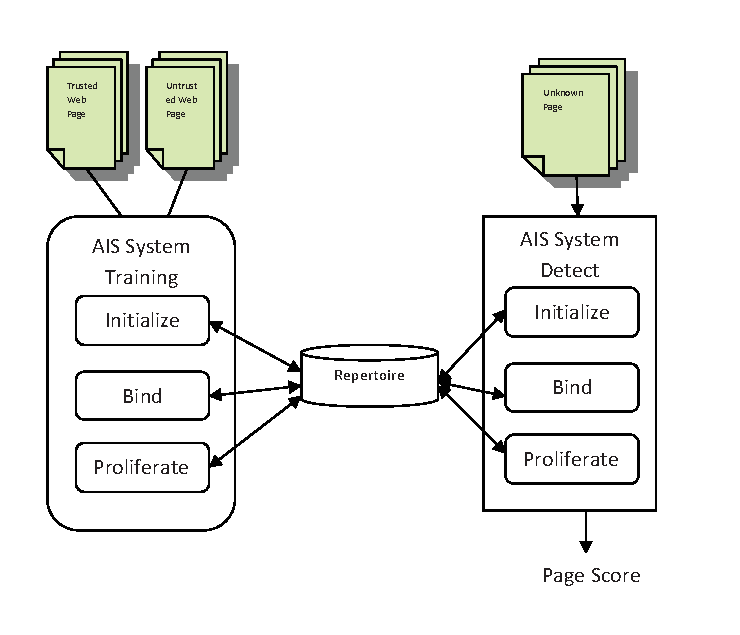
\includegraphics{arch.eps}}
\caption{AIS-based Trust Computing system}
\label{fig:arch}
\end{center}
\vspace{-20pt}
\end{figure}

\subsection{Result}
We trained our Immune System using the data in GOV WTX001 data set\cite{WTX}. We did not train on the whole data set due to the limited time for this project. For untrusted web site, we trained our system over 120000 web pages listed in \cite{WEBSPAM-UK2007}. Then we tested our system over 219 trusted web pages and 200 untrusted web pages in \cite{WEBSPAM-UK2007}. The result is presented in Table \ref{table:result}.
\begin{table}[t]
\renewcommand{\arraystretch}{1.3}
\caption{\small Ais-based Trust System Result}
\label{table:result}
\centering
{\scriptsize
\begin{tabular}{ccccc}
\hline
Number of Pages & Page Type & Trusted Pages & Untrusted Page & False \%\\
\hline
219 & Trusted & 201 & 18 & 8.2\%\\
200 & Untrusted & 38 & 162 & 19\%\\
\hline
\end{tabular}
}
\end{table}

\section{Conclusion and Future Works}
In this paper, we describe our trust classification model inspired by artificial immune system. Applying artificial immune system classifier to categorize web pages according to their link structure is work in progress. In this approach, we have more general view in way that we consider the whole web as a system. Each web page plays a role of t-cells. \\
We also need to run more evaluation. We already implemented the Naïve Bayesian algorithm. We are going to run this algorithm in our data set and compare the results with our immune based trust classifier.\\
The cross regulation algorithm that we currently used can be more complicated. For example, currently we did not consider the death rate for t-cells. We think we may be able to use different type of t-cells that can live longer. Or since trust is dynamic concepts, it can change over the time. We think about using a model that can provide us this kind of dynamic update. \\
The most interesting continuation of this research in our perspective is presenting multi level trust classifier based on immune system. In This way we can look at trust as fuzzy concept and calculate trust specifically for each attribute of the web pages.  \\
As more web pages employ java script to enhance the intractability, java script introduce more security issues. Well the understanding the semantic of java script would be difficult. In \cite{kruegel03:webanomaly}, a script analysis way was proposed, but understanding the semantics of java scrip would be complex, we are thinking about using AIS system to analysis java scripts and differentiate that trusted and malicious java script code.

\acknowledgements{Acknowledgements belong here.}

\begin{thebibliography}{99.}%
\bibitem{blaze} M. Blaze, J. Feigenbaum and J. Lacy, “Decentralized trust management,” IEEE
symp. on security and privacy, pp. 164-173, 1996
\bibitem{surveyInternt}T. Grandison and M. Sloman, "A Survey of Trust in Internet Applications,"IEEE Communications Surveys and Tutorials, vol. 3, no. 4, pp. 2-16, 2000.
\bibitem{AIS} E.  Burke and G. Kendall, “Artificial immune systems,”  chap 13,  search methodologies: Introductory tutorials in optimization and decision support techniques. 
\bibitem{mitchell}N. Li, J. Mitchell and W. Winsborough, “Design of a role-based trust-management
framework,” in Proc. of IEEE symp. on security and privacy, 2002.
\bibitem{mitchell1} N. Li and J. Mitchell, “RT: a role-based trust-management framework,” in DARPA
information survivability conf. and exposition (DISCEX), Apr. 2003.
\bibitem{mitchell3} ] N. Li, W. Winsborough and J. Mitchell, “Distributed credential chain discovery in
trust management,” j. of computer security, vol. 11, no. 1, pp. 35-86, 2003.
\bibitem{reputationWeb} K. Lin   H. Lu,   T. Yu   C. Tai, "A reputation and trust management broker framework for Web applications,"EEE '05. Proceedings of e-Technology, e-Commerce and e-Service, pp. 262-269, 2005.
 \bibitem{trustpolicy} Y. Chu, J. Feigenbaum, B. LaMacchia,  P. Resnick, M. Strauss, "trust management for Web applications," J. of computer networks and ISDN systems, vol. 29, pp. 953-968, 1997. 
\bibitem{Winslett} M. Winslett, T. Yu, K. E. Seamons, A. Hess, J. Jacobson, R. Jarvis, B. Smith, and L.
Yu, “Negotiating trust on the Web,” IEEE internet computing, pp. 30-37,vol. 6, no.
6, 2002.
\bibitem{Winslett2} M. Winslett, T. Yu, K. E. Seamons, A. Hess, J. Jacobson, 
R. Jarvis, B. Smith, and L. Yu., " The TrustBuilder architecture for trust negotiation," IEEE Internet Computing, 6(6), 2002.
\bibitem{Squicciarini} A. C. Squicciarini, E. Bertino, et al, “Achieving
Privacy in Trust Negotiations with an Ontology-Based
Approach”, Transaction of dependable and Secure
Computing, vol. 3, no. 1, 2006, pp. 13-30.
\bibitem{Koshutanski} H. Koshutanski and F. Massacci. Interactive trust 
management and negotiation scheme. In Workshop on 
Formal Aspects in Security and Trust, Aug. 2004.
\bibitem{Winsborough} W. Winsborough, K. Seamons, and V. Jones. Automated
trust negotiation. In DARPA Information Survivability Conference
and Exposition, volume 1, pages 88ñ102, 2000.
\bibitem{Winsborough2} W. H. Winsborough and N. Li. Towards practical automated
trust negotiation. In Proceedings of the 3rd International
Workshop on Policies for Distributed Systems and
Networks, pages 92-103, 2002.
\bibitem{competent} M. Smith and M. DesJardins, " Learning to trust in the competence and commitment of agents," J. of 	Autonomous Agents and Multi-Agent Systems, pp. 36-82, 2008. 
\bibitem{experince} K. Fullam andK. Barber, "Dynamically Learning Sources of Trust Information: Experience vs. Reputation," Proceedings of the Sixth Intl. Joint Conf. on Autonomous Agents and Multiagent Systems, pp. 1062-1069, 2007.
\bibitem{statistical} A. REttinger, M. Nickles, V. Tresp, "A statistical relational model for trust learning," International Conference on Autonomous Agents,  pp.763-770, 2008. 
\bibitem{inittrust} A. Rettinger, M. Nickles, and v. Tresp,  "Learning Initial Trust Among Interacting Agents," LNCS Cooperative Information Agents XI, pp. 313-327, 2007.
\bibitem{taskspecific} I. Erete, E. Ferguson, S. Sen, " learning task-specific trust decision," Proceedings of the 7th international joint conference on Autonomous agents and multiagent systems , vol. 3,  pp. 1477-1480, 2008.
\bibitem{WTX}
Government data set.
\newblock \url{http://acsys.anu.edu.au/}, 2000.

\bibitem{WEBSPAM-UK2007}
Yahoo! research: Web spam collections.
\newblock \url{http://www.yr-bcn.es/webspam/datasets/uk2007/}, 2007.

\bibitem{Common}
The most common english words.
\newblock \url{http://www.world-english.org/english500.htm}, 2009.

\bibitem{Porter}
S.E.~Robertson C.J.~van Rijsbergen and M.F. Porter.
\newblock New models in probabilistic information retrieval.
\newblock {\em British Library Research and Development Report}, (5587), 1980.

\bibitem{aisLearning} J.D. Farmer, N. H. Packard, A. S. Perelson, "The immune system, adaptation, and machine learning," Phisica D, vol. 2, pp. 187-204, 1986. 
\bibitem{Forrest1} P. D'haeseleer, S. Forrest, and P. Helman, "An Immunological Approach to Change Detection: Algorithms, Analysis, and Implications,"  In Proceedings of the 1996 IEEE Symposium on Computer Security and Privacy, 1996.
\bibitem{Al1} A. Abi-Haidar and L.M. Rocha,  "Adaptive Spam Detection Inspired by the Immune System". In:  Artificial Life XI: Eleventh International Conference on the Simulation and Synthesis of Living Systems, pp. 1-8, 2008.
\bibitem{Al2} A. Abi-Haidar and L.M. Rocha, "Adaptive Spam Detection Inspired by a Cross-Regulation Model of Immune Dynamics: A Study of Concept Drift," 	Artificial Immune Systems, pp. 36-47, 2008.
\bibitem{spam} G. B. Bezerra, T. V. Barra, H. M. Ferreira, H. Knidel, L.  Castro and F. J. Von Zuben, "An Immunological Filter for Spam," LNCS 	Artificial Immune Systems, pp. 446- 458, 2006. 
\bibitem{Forrest2} J. Balthrop, F. Esponda, S. Forrest and M. Glickman. In W. B. Langdon, E. Cantu-Paz, K. Mathias, R. Roy, D. Davis, R. Poli, K. Balakrishnan, V. Hanovar, G. Rudolph, J. Wegener, L. Bull, M. A. Potter, A. C. Schultz, J. F. Miller, E. Burke and N. Jonaska, editors. "Coverage and Generalization in an Artificial Immune System." Proceedings of the Genetic and Evolutionary Computation Conference. (GECCO 2002), Morgan Kaufmann. New York, pp. 3-10 (2002).
 \bibitem{LISYS} J. Balthrop, S. Forrest, and M. Glickman, "Revisiting LISYS: Parameters and Normal Behavior," Proceedings of the 2002 Congress on Evolutionary Computation  (2002).

\bibitem{carneiro} J. Carneiro, K. Leon, I. Caramalho, and R. Gardner “When there is not a crowd: a cross regulation model of the dynamics and repertoire selection of regulatory CD4+ T cells,” Immunological reviews, vol. 216, pp. 48-68, 2007.

\bibitem{kruegel03:webanomaly}
C.~Kruegel and G.~Vigna.
\newblock {Anomaly Detection of Web-based Attacks}.
\newblock In {\em Proceedings of the $10^{th}$ ACM Conference on Computer and
  Communication Security (CCS '03)}, pages 251--261, Washington, DC, October
  2003. ACM Press.
\end{thebibliography}

%%\bibliographystyle{plain}
%%\bibliography{bib}
\end{document}
